\documentclass[procedia]{easychair}

\usepackage{graphicx}
\usepackage{float}
\usepackage{url}
\usepackage{xspace}
\usepackage{enumitem}
\usepackage{subcaption}

\def\procediaConference{Thinking-Understanding approach with small data in a world of Big Data(BICA 2015)}


\title{Thinking-Understanding approach with small data in a world of Big Data}
%TUSM: Thinking-Understanding approach with small data in a world of Big Data}

\author{
Alexander Toschev\inst{1}
\and
Max Talanov \inst{1}
}

\institute{
Kazan Federal University, Russia.
}

\authorrunning{A. Toschev, M. Talanov, \ldots}
\titlerunning{TUSM: \ldots}

\begin{document}

\maketitle

\begin{abstract}
Observing tsunami of articles for new IT direction: "Small Data", including titles: "Forget Big Data, Small Data is the Real Revolution" and "How To Create Incredible Customer Service Through The 'Small Data' Advantage" for example on Forbes.com, we face the rising interest of the human analogous data analysis. The challenging moment is the number of instances in disposal that we can not use statistical or machine learning methods instead neurobiologically inspired methods should be used. Using the model of mental activities known as cognitive architecture is the main tool to overcome the small data problem, and there is no "silver bullet" analysis method as humans are too multilateral in analysis and decision making that Small Data analysis framework is to be developed.
At the moment there a lot of systems that can perform search for data in large amount of files. However, result still should be reviewed by human expert. But what if another system can calculate report based on found information with comparison of information.

\keywords{Cognitive architecture, Affects, Emotions, Emotion Modeling, Cognitive Science}

\end{abstract}

\section{Introduction}

Several last years big data was in the center of interest of and thus data scientist enjoyed the data centralization and integration in huge volumes. There are magnificent examples of big data analysis in use: Watson by IBM, "Human brain project", "Blue brain project". Slight shadow of hesitation run thought the face of some specialists asking the question do our brain work the same way and if not why not? It seems to be pretty good to process this amounts of exabytes and roll out resulting report. Unfortunately we have to live in the real time and usually we do not have time to run the exhaustive analysis, we have to make decisions here and now. That's why the other mechanism of quick decision making evolved. The other application field is the analysis of the big-data reports, currently there are human analysts that are doing this work in every industry for every major company for every more or less interesting filed and set of parameters.Still "the shoemaker's children go barefoot" in general we are unable to solve any even simple problem that somehow is connected to human understanding.

But demand is really high current robotics systems are not able of doing more or less reasonable reactions in complex social environment, analytical systems are capable of decision support in environment of the exabytes of data. IoT demands distributed decision making in real time that puts us into position of inventing of new methods and approaches.

First fact that biased our mindset is that brain contributes the 20 Watts only and still capable of much more that modern computational systems. Second is the decision making is done with much less data required for the training and still we tend to rely on human decision making much more than on machine with big data analysis. In medicine there are decision support systems that leaves final decision to human doctor.

The problem: Currently data processing is dominated by statistical methods, which has the following limitations:

(1) The required data is not available -- e.g., the prior distribution required by the Bayesian approach cannot be effectively determined in many situations. It has been point out by many researchers that probability theory cannot handle ignorance ("I don't know") naturally.

(2) The required data is not available at the same moment -- For systems that work in real time or handle online information, the data come prom time to time, which statistical methods usually cannot handle incremental revision very well.

(3) The available data are inconsistent -- When data comes from multiple sources or at different periods, it is common that they support conflicting or contradicting conclusions. Since statistical methods usually assume each event has a unique probability (though it can be unknown), this "data fusion" problem has not got a widely accepted statistical solution.

(4) Statistical methods often take a long time to compute, which is not always affordable in practical situations where problems demands real-time solutions.

(5) Since statistical methods usually works on a constant sample (or propositional) space, they normally can only evaluate given hypotheses, but cannot generate hypotheses. For many practical problems, it is very unnatural to assume all the candidate answers are known at the beginning.
%\subsection{Contributions}
The main contribution of this paper is twofold:
%\begin{itemize}
% \item
% We have
i) extending the neuro-psychological three dimensional model of affects ``Cube of emotions''\cite{lovheim2012}
with mapping to parameters of von Neumann machine and computational system decision making;
% \item
%We have
ii) implementing neuromodulation mechanisms of dopamine in spiking neural network NEST
\footnote{\url{http://www.nest-initiative.org/}} framework, thus one axis of three dimensional model and
indicated the connection of one affect --- fear --- with the computational power load, learning and storage.
%\end{itemize}

The remainder of the paper is organized as follows: problem description is provided in  Section \ref{sec:problem},
while  our emotion-based approach, NEUCOGAR, is presented in  Section \ref{sec:neucogar}, and detailed analysis is provided
in Section \ref{sec:val} with experiment description and results discussion.
Section \ref{sec:concl} closes the paper with some remarks and conclusions.

\section{The problem}
\label{sec:problem}

Recently, a new generation of cognitive scientists and roboticists proposed a turnover: by one hand, emotions
are a fundamental part of the cognitive processes (attention, motivation, strategy selection, mood disposal,
reaction, invention, among a long list); on the other hand, the intrinsic relationship between minds and bodies led to
the birth of embodied cognition or grounded cognition\cite{Barsalou2008}.
This allowed the emergence of a second and powerful wave of cognitive and robotics experts lead by people like
Rodney Brooks \cite{Brooks1991, Brooks1995} or James DeLancey (Robotics) \cite{Delancey2001}, Andy Clark (Philosophy)
\cite{Clark2003},
Antonio Damasio \cite{Damasio1999}, Ramachandran \cite{Ramachandran2004}, or Rizzolatti (Neurology) \cite{Rizzolatti2004}.

In the middle of this cognitive revolution that led to embodied robotics, enactive cognition or morphological
computation ideas, an important discipline emerged as a main reference: Neuroscience.
Neuroscientists revolutionized the discipline with data coming from \emph{in vivo} scanned brains (by EEG, fMRI)
and brought relevance to the emotional processes into the whole system.  Some authors as a consequence attempted
explanations on the emergence of consciousness (Damasio, Llin{\'a}s \cite{Lli}). Therefore, researchers in AI
or cognitive science started to introduce ideas about emotional processing.

Once explained the crucial role of grounded and emotional aspects in cognitive architectures, we assume the
L{\"o}vheim model as a reference for our own architecture. L{\"o}vheim \cite{lovheim2012} based his theory on
a three-dimensional model of emotions and monoamine neurotransmitters (\textit{serotonin, dopamine, noradrenaline}).
The vertexes of
the model are affects, as defined by the Tomkins theory, which describes eight basic emotions
\cite{kelly2009}. Tomkins labeled with one word for the emotion when it was of low intensity and
another word for the same emotion at a higher intensity. Tomkins referred to basic emotions as ``innate affects''
where affect \cite{tomkins1962, tomkins1963, tomkins1991}, in his theory, stands for the ``strictly biological portion of emotion".
According to his theory, these are the eight basic emotions: \textit{Enjoyment/Joy, Interest/Excitement,
Surprise, Anger/Rage, Disgust, Distress/Anguish, Fear/Terror and Shame/Humiliation}.
Some of these emotions are managed only by the internal processes of the individual, but some other
are intrinsically related to social interactions.

\section{Our cognitive affective architecture: NEUCOGAR}
\label{sec:neucogar}

In this section we present our novel approach to artificial cognitive architectures, the Neuromodulating Cognitive
Architecture (NEUCOGAR). The idea is to create a mapping of monoamine neuromodulators to emotional states
applied to computational system parameters. Our work starts from the following considerations:

\begin{enumerate}
\item Emotions are natural and necessary modulators, reinforced and modeled at the same time by social external
factors or even internal thoughts.
\item Monoamine neuromodulators are the physical mechanism by which emotional responses
are triggered and modulated within cognitive systems like humans \cite{marsella2003, marsella2010}.
\item
Several modular models are available: Geneva emotion wheel, Plutchick's ``Wheel of emotions'' \cite{plutchik2001},
or L{\"o}vheim ``Cube of emotion'' \cite{lovheim2012}, among others. All of them identify different
strategies, the basic emotions and how dynamic transitions among them are created \cite{gratch2005}.
\end{enumerate}

Stemming from this simple points, our work is focused on modeling the mapping of impacts of monoamine
neuromodulators on human brain into the computational processes of modern computers.
We propose the approach to correlate biochemical influence of monoamines such as \textit{dopamine, serotonin,
and noradrenaline}, involved in affective processing of cortical, limbic and other subsystems of human brain
with computational processes: \textit{computational power, memory distribution, learning and storage, or decision
making} that take place in computational systems.

We have implemented the dopamine neuromodulation for validation of the proposed model of computational
affects to reimplement the fear affect in the computational system and check one axis of our model.

\subsection{NEUCOGAR in details}
\label{sec:analysis}

\begin{figure}
    \centering
    \includegraphics[width=0.8\columnwidth]{figure3_cube_of_parameters_top}
    \caption{Computing system emotion parameters}
    \label{fig:cube}
\end{figure}

%NEUCOGAR is based on L{\"o}vheim (2012) model on neurotransmitters.
In Figure \ref{fig:cube} a revised version of the cube of emotions
%is shown as
model, originally introduced by Hugo L{\"o}vheim in his seminal paper on the topic \cite{lovheim2012}, is depicted.
The information on the cube is adapted to the computing domain and extended to include the parameters above discussed such as: computing power, memory and learning.
%Fig. \ref{fig:cube}
It represents the link bridging neuroscience and psychology with concepts of computational and AI systems.
%thus  specialists.
This paper aims at building a common understanding between these three worlds and possibly fostering a productive cooperation among specialists of all these fields.

Low level influence of affects on brain (cellular or neuronal) provides fundamental base for our affective
computation model. We draw an analogy between computational processes in computer and neurotransmission in brain, simulating
biochemical influence of neuromodulatory systems on neurons and translating them into the computational processes
of a machine. Especially interesting from our perspective is \cite{fellous2004}, where the role of dopamine,
serotonin and their impact in emotional context (of mammalian brains) is discussed and it could be considered as
one of the basis for our work in the neuromodulation domain:

\textit{Dopamine}.
Dopamine appears to play a major role in motor activation, appetitive motivation, reward processing and cellular
 plasticity, and might be important in emotion.

According to L{\"o}vheim cube of emotions dopamine is associated with ``[r]eward, reinforcement, motivation''.
From computational system perspective we interpret dopamine as playing a role in: reward processing thus in
decision making, working memory --- memory distribution and storage in computing system, motivation --- decision making.

\textit{Serotonin}.
``Serotonin has been implicated in behavioral state regulation and arousal, motor pattern generation,
sleep, learning and plasticity, food intake, mood and social behavior''.
Serotonin plays a crucial role in the modulation of aggression and in agonistic social interactions in many animals.

L{\"o}vheim associates serotonin with ``[s]elf confidence, inner strength, and satisfaction''. Thus
our interpretation of influence of serotonin system looks like: decision making of the system is influenced by serotonin,
confidence and satisfaction as coloring of the knowledge is impacted by serotonin too, this way serotonin should influence
training of machine and storage of the information learned.

\textit{Noradrenaline}.  L{\"o}vheim cube of emotions emphasizes the noradrenaline role in: ``Attention,
vigilance, activity''. Then he describes the role of noradrenaline: ``... noradrenaline has been coupled to the fight or
flight response and to stress and anxiety, and appears to represent an axis of activation, vigilance and attention''.

The decision making is influenced by alertness effect of noradrenaline reducing number of options in the observation,
and possibly making system use more risky choices.


\subsection{From emotions to computing system}

The idea behind the mapping of neuromodulators to computational systems' parameters stands
in creating a link between the Von Neumann architecture (abstractly a Turing
Machine) and the neuroendocrine system.

It has been historically thought
that AI systems could be built on top of traditional computational architectures
provided enough computational power and memory resources were in place and adequate
algorithms were available. It was just a matter of time, money and technology. After the initial
excitement to this regard (mainly in the 50s of last century) and numerous
failures in reaching the desired results, it has been lately hypothesized that this may
not be the case. Technically, the neuroendocrine system may not be a Turing Machine,
though the functioning is not fully understood at the moment. In particular, it is not clear
whether higher functions performed by humans, as for example consciousness, are epiphenomena
of the brain itself or not.

Despite of this, and accepting the fact that we may not be able to model the full neuroendocrine
system into the Von Neumann architecture, parallels can still be built and relationships
between the two can help develop systems for specific purposes. This is the case of L{\"o}vheim cube of emotions
where analogies are only built on top of it
in relation to \textit{dopamine, serotonin and noradrenaline} levels. Simulation
of emotions plays a major role in several IT and AI field, not last in the robotics. The ability of a
system to feel emotions like, for example, \textit{fear, interest or joy} can
trigger behaviors that were not possible in the era of \textit{unemotional machines}.

\textit{Moral machines} may emerge from such a research strand, i.e. machines with in-built
perceptions of ``right'' and ``wrong'' and unable to harm humans (like in Asimov's ``Three Laws of Robotics'').
It is well-know as \textit{pet therapy} is beneficial in
helping patients to recover from or cope with health problems or a mental disorders. Emotional
machines will provide enormous support in such a cases and replace animals when they have to operate
in hostile environments or simply when it is more cost effective. More generally, automated desk-service
or call center may be able to cope with customers needs maintaining the appearance of human touch and
providing continuous service without discontinuity due to tiredness.

As the human brain as a whole reacts to changes in the neuromodulator and hormonal levels, the model
presented in this paper offers a ground for simulations of emotions in the Von Neumann architecture
(with the clear understanding that, most likely, not every brain function can be reproduced in the same
way). This mapping is clearly not sufficient: proper algorithms need to be developed to reproduce higher
functions on top of the \textit{``hormonal reactive machinery''}. These algorithms will monitor CPU activity
and memory allocation in order to track (simulated) \textit{hormonal and neuromodulators levels} and react accordingly.

Higher functions of the brain like consciousness and proactivity (the ability of not reacting in the short term
to immediate physiological responses) may possibly be simulated on top of basic functions. However, this
still remains an unproven hypothesis needing accurate investigation. If such higher functions are indeed
epiphenomena of the brain (or endocrine systems) is still under debate in several scientific communities.

According to their nature  we can split computing system parameters in three groups:
processing, memory and storage.
More specifically, the parameters taken into account are:

\begin{description}
 \item[Computing power load]: overall load of the computational system is influenced by dopamine and
serotonin that makes cortex fire spikes more actively.
 \item[Computing power redistribution]: distribution and priority of parallel process or load balancing,
is measured by noradrenaline.
 The higher the level of noradrenaline the more computing power must be concentrated on current activity
(neuromodulator regulating attention).
 \item[Working memory (short term) distribution and concentration] is impacted by noradrenaline (attention).
 \item[Storage management (long term memory)] is impacted by both serotonin and dopamine, higher concentrations of
both neuromodulators makes system better remember a stimulus. In general, strong emotions generate more persistent
memories.
\end{description}

\subsection{Mapping to other domains}

\textit{Learning} is another parameter (not inherited from Von Neumann architecture)
identifying a training and a new information gathering. It is impacted by serotonin and
dopamine: dopamine plays major role in activation of previously remembered patterns
and serotonin in pattern generation.

\textit{Decision making} group represents parameters
and coloring (tagging, flagging)
of the trained information exploited during the decision making processes. Confidence
impact on decision making is one of the most obvious and important, even the selection
of the information is done taking in account how system is confident in this information.
\textit{Satisfaction} is one of most important flags involved in reward system usually making
system to select most satisfactory/pleasurable actions (approaches). The \textit{motivation}
drives system to make most desirable selections and heavily influences selections
of further activities. The \textit{number of options} to process and \textit{inclination to risky}
actions are linked to noradrenaline stressful situation alertness; both of them
make system do quick decisions with tendency to risk. \textit{Confidence and satisfaction} of the system
is influenced by serotonin.
Systems are more \textit{motivated} under the influence of dopamine. Systems tend to choose
\textit{risky actions} under the influence of noradrenaline.
Noradrenaline makes system
consider a smaller number of options in width and depth to be processed during deliberation.

%\begin{description}
%\item [Confidence]: serotonin
%\item [Satisfaction]: serotonin
%\item [Motivation, wanting]: dopamine
%\item [Number of options to process]: noradrenaline
%\item [Risky choices inclination]: noradrenaline
%\end{description}

Decision making is principally done in deliberation and learned reaction layers
of ``Model of six'' \cite{minsky2007} through parameters such as confidence,
satisfaction, risky choices inclination, which are used to highlight actions
stored (remembered). This mapping is exhaustively described in
%``Computational emotional thinking and virtual neurotransmitters''
\cite{talanov2014} and could be used as a low level model of emotional processes
and also as a basic framework for the emotion enabled systems.

\section{Preliminary evaluation and validation}
\label{sec:val}

\subsection{Experiment description}

The experiment is validation of a dopamine neuromodulation and its influence on a Cerebral
cortex thus thinking processes and thus computational processes.
We made the general assumption that thinking processes are analogous,
or could be expressed, as computational processes. We have implemented a dopamine pathway published by
Albin et al.\cite{dopa_albin} with some extensions for a feed-back loops and additional
connections according to modern discoveries in neuroscience \autoref{fig:BG_advanced}.
The dopamine neuromodulation is influenced by a Substantia nigra compacta(SNc) that produces a dopamine
and projects to a Striatum.
Mammalian Striatum consists of neurons with different dopamine receptors: D1 and D2
that implement the balancing between direct and indirect pathways (depicted below
on \autoref{fig:BG_advanced}) due to their heterogeneous sensitivity to dopamine
neurotransmitter.

%\noindent
The direct pathway is
\textit{Cerebral cortex} (stimulate) $\to$ \textit{Striatum} (inhibit) $\to$ \textit{complex SNr-GPi} (Thalamus is less inhibited) $\to$ \textit{Thalamus} (stimulate) $\to$ \textit{Cerebral cortex} (stimulate) $\to$ \textit{muscles and etc.}

%\noindent
The indirect pathway is
\textit{Cerebral cortex} (stimulate) $\to$ \textit{Striatum} (inhibit) $\to$ \textit{GPe} (STN is less inhibited) $\to$ \textit{STN} (stimulate) $\to$ \textit{complex SNr-GPi} (inhibit) $\to$ \textit{Thalamus} (is less stimulated) $\to$ \textit{Cerebral cortex} (is less stimulated) $\to$ \textit{muscles and etc.}\\

\begin{figure}
\center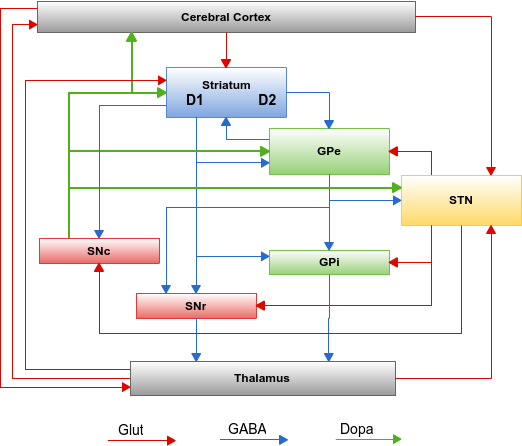
\includegraphics[width=0.6\textwidth]{dopamine_pathway}
\caption{Basal ganglia circuits: Thalamus; Cerebral cortex; Striatum; GPe\ ---
Globus pallidus external; GPi\ ---- Globus pallidus internal; STN\ --- Subthalamic nucleus; SNc\ --- Substantia
nigra compacta; SNr\ --- Substantia nigra reticulata.
Red arrows identifies excitation, blue --- inhibition, green --- modulation connections.}
\label{fig:BG_advanced}
\end{figure}

\subsection{Results}

The dopamine neuromodulation is caused by modeled Substantia nigra compacta that increases spiking activity of the Striatum and
accordingly it balances to the direct pathway from the indirect one, which entails
a increased spiking activity in the Thalamus see \autoref{fig:thalamus_activity}
and later on the Cerebral Motor cortex, see \autoref{fig:cortex_activity}.
In other words increased spiking activity indicates the \textit{increased processing power consumption} of the system.
The \textit{motivation} of the system is regulated by dopamine in ``wanting'' pattern and inclination to use more dopamine
colored decisions in future.
The \textit{learning} is improved due to the increase of spiking activity in the Thalamus that is having feedback loop to
the Cerebral cortex and consolidates a new information according to the Hebbian theory of neuron adaptation to spiking
activity \cite{hebb1949}, taking in account the influence of the dopamine neuromodulating system.
Listed above deliberations indicates the principle correctness of the hypothesis presented earlier in the Section \ref{sec:neucogar} and on \autoref{fig:cube} along to only one axis of a dopamine.

\begin{figure}
\centering
%\begin{subfigure}{.49\textwidth}
  \centering
  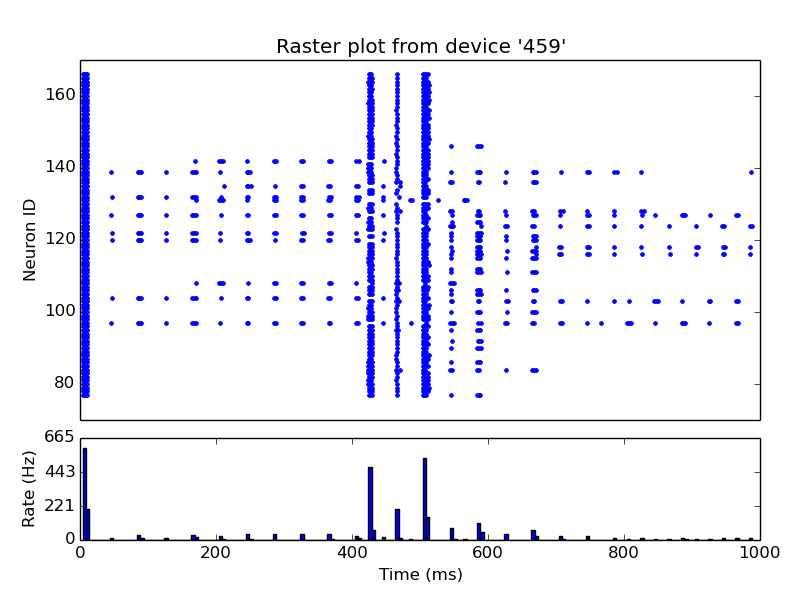
\includegraphics[width=0.9\textwidth]{spikes_thalamus}
  \caption{Increased spiking activity on the Thalamus from 400 to 600 ms}
%\end{subfigure}
\label{fig:thalamus_activity}
\end{figure}

\begin{figure}
%\begin{subfigure}{.49\textwidth}
  \centering
  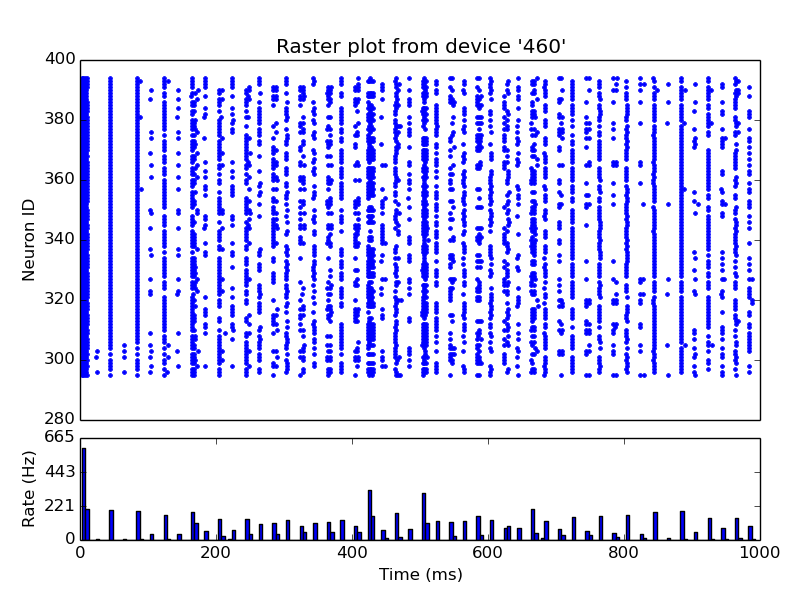
\includegraphics[width=0.9\textwidth]{spikes_motorcortex}
  \caption{Increased spiking activity on the motor cortex from 400 to 600 ms}
%\end{subfigure}
\label{fig:cortex_activity}
\end{figure}

\section{Conclusions}
\label{sec:concl}

According to modern scientific picture  and latest results of a trans-disciplinary view on cognition
the embodiment of cognitive processes can be affirmed.
The mind/bodily management is related
to emotional signals that capture, process and classify data inputs (external or
internal, you need to remember the multi-modality of emotions) and allow responses.
The fundamental role of emotions in cognitive processes is quite clear at the moment even for
artificial cognitive systems.

We propose the neurobiologically inspired cognitive architecture for the simulation of the affects in
a computational system.
Our approach is innovative for several reasons:

\begin{itemize}
\item We need not running a whole brain simulation in order to achieve a functional
artificial cognitive system, and this allow us to avoid the still existing and deep
uncertainties between brain structure and performance
(at this historical moment, brain researchers are at the same point that genetic
biologists starting to decode the genome: with a lot of information, in fact too much,
but without meaning).
\item We are not qualitatively imitating the surface of the emotional syntax of
human brains and bodies, but instead we are suggesting a new approach that is
rooted in the neuromodulators syntax, the key piece of brain emotional and
cognitive processes.
\item This functional approach allows generation of more dynamic systems
that add cognitive power beyond the basics of classic weights, thresholds or
valences, providing options to build a cognitive architecture that generates several faces
of emotional interactions such as moods, attitudes, emotional memories or affective states.
\end{itemize}

The NEUCOGAR provides the proper background to the implementation of emotional elements into the whole system,
acting as the basic piece of regulation, and not as an attached module with emotional
contents. This architecture allows to apply it smoothly from the scratch (the artificial
neuron or unit of processing) to the superior layers of specialized cognitive processes
(like memories, processors). In this sense, NEUCOGAR is a whole artificial cognitive
system that simulates the basic running of bodily emotional systems, following
a modular architecture that is put together and ruled by the same
emotional cyber-neuromodulators.

The validation of the NEUCOGAR is complex task that involves use of spiking neural network
NEST\footnote{\url{http://www.nest-initiative.org/}} and creation
of proper brain cortical and subcortical areas and connections. We have managed to validate only one axis
of the NEUCOGAR model --- the dopamine axis, because it has been most researched
at the moment and thus easiest to implement. This validation indicated principal
correctness of the approach to simulate emotions in the form of inborn affects
in a computational system.

\subsection{Future work}

We consider adding serotonin pathways as the most important extension of current implementation.
That will allow validation of up to 4 affects: joy, fear, disgust, humiliation,
and overall will make the model from one-dimensional to bi-dimensional.
Further enhancement with noradrenaline will provide the 8 basic affects that
could be used as the base for the implementation of the infant emotional cognitive
architecture as well as be helpful for the emotion recognition, evaluation and measurement.

\section*{Acknowledgments}

Partial support for this research was received by the Spanish Government's DGICYT research project: FFI2011-23238, ``Innovation in scientific practice: cognitive approaches and their philosophical consequences" and by the Russian Ministry of education and science (agreement: 14.612.21.0001, ID: RFMEFI61214X0001).


\bibliographystyle{plain}
\bibliography{neucogar}

\end{document}
